\chapter{Performance of Our Driver}
\label{chap:performance}
To compare the performance of our driver to BitLocker and VeraCrypt, we conducted several experiments measuring the read rates for both sequential and random access. Preliminary tests were done in a virtual machine, and after some optimizations, we tested more extensively on real hardware. Finally, we also measured how the read rates behave over time.

\section{Experimental Setup}
\label{chap:performance.setup}
Both the setup for the virtual machine and the real hardware will be described in this section. They are mostly the same, so unless stated otherwise, the contents in this section apply to both.

Both configurations used a fresh Windows 10 build 19043.928 install. The virtual machine ran in Oracle VirtualBox 6.1.22 with 8 GiB of virtual RAM (backed by 16 GiB DDR4 RAM), 4 virtual cores (backed by a Intel Core i7-7700K), and two virtual disks (backed by a 250 GB Samsung SSD 850 EVO). The real machine had 8 GiB DDR3 RAM, an Intel Core i7-3770 quad core with simultaneous multithreading, and a 233 GiB SanDisk SDSSDH3250G.

For each encryption technique featured in our benchmarks we created a separate 5 GiB FAT32 volume on the same disk, as shown in \autoref{fig:performance.setup.disklayout}. Every encrypted volume contained the same file, \texttt{random.bin} (4 GiB of random data). We configured BitLocker to use the new AES-XTS mode, all other settings were left unchanged. For VeraCrypt, we also used AES-XTS with SHA-256 and also mounted the volume as read-only after copying the \texttt{random.bin} file to it.

\begin{figure}[htb!]
	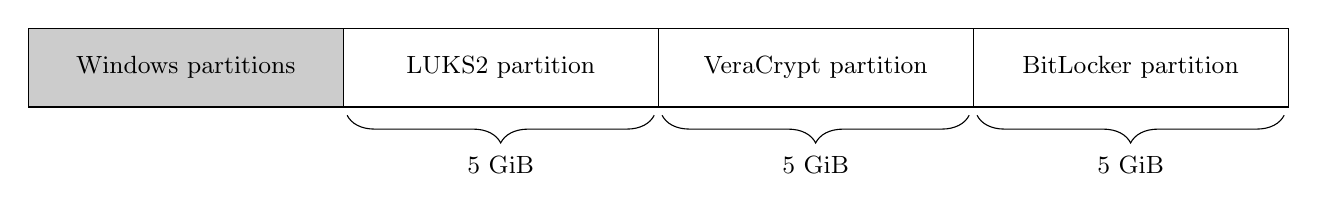
\begin{tikzpicture}
		\draw [fill={gray!40}] (0, 0) rectangle (4, 1);
		\node [anchor=center] at (2, 0.5) {\small\makecell{Windows partitions}};
		\draw [fill=white] (4, 0) rectangle (8, 1);
		\node [anchor=center] at (6, 0.5) {\small\makecell{LUKS2 partition}};
		\draw [fill=white] (8, 0) rectangle (12, 1);
		\node [anchor=center] at (10, 0.5) {\small\makecell{VeraCrypt partition}};
		\draw [fill=white] (12, 0) rectangle (16, 1);
		\node [anchor=center] at (14, 0.5) {\small\makecell{BitLocker partition}};

		\draw [decorate, decoration={brace, amplitude=10pt, mirror}, yshift=-3pt]
		(4.05, 0) -- (7.95, 0) node [black, midway, yshift=-18pt] {\small 5 GiB};
		\draw [decorate, decoration={brace, amplitude=10pt, mirror}, yshift=-3pt]
		(8.05, 0) -- (11.95, 0) node [black, midway, yshift=-18pt] {\small 5 GiB};
		\draw [decorate, decoration={brace, amplitude=10pt, mirror}, yshift=-3pt]
		(12.05, 0) -- (15.95, 0) node [black, midway, yshift=-18pt] {\small 5 GiB};
	\end{tikzpicture}
	\caption[
		Volume layout for our experiments
	]{
		Volume layout for our experiments. This is the layout of the real hardware SSD. The virtual machine had a virtual disk for the Windows installation and another one for the three encrypted volumes.
	}
	\label{fig:performance.setup.disklayout}
\end{figure}

To compare the performance of the different drivers, we used version 3.27 of the \texttt{fio} command line tool \cite{Fio} to read from the three copies of \texttt{random.bin}, using different access patterns. Each run of \texttt{fio} is called a \emph{job}, and the configuration for a job is stored in a \emph{job file}. We maintained a different job file for each of the three encryption technologies. \autoref{fig:performance.setup.fiojobfile} describes the different parameters that we used and shows the configuration for \texttt{luks2flt}. \texttt{fio} allows the user to specify which I/O engine to use. The default on Windows is the native asynchronous I/O API, which is what we used.

\begin{figure}[htb!]
	\begin{inicode}
[luks2flt]
filename=L\:\random.bin
thread
iodepth=${IODEPTH}
numjobs=${NUMJOBS}
rw=${MODE}
bs=${BLOCKSIZE}
	\end{inicode}
	\caption[
		\texttt{fio} job file for \texttt{luks2flt}
	]{
		\texttt{fio} job file for \texttt{luks2flt}. It defines one job called \texttt{luks2flt}. The \texttt{filename} option's value is the only one that depends on the used driver; the rest of the configuration is the same for BitLocker and VeraCrypt. The \texttt{thread} option means that \texttt{fio} will create threads instead of processes to run jobs (which is always done on Windows, but when not specifying this option, the user is warned about this behaviour). The \texttt{iodepth} parameter controls how many I/O operations \texttt{fio} will try to submit before waiting for the completion of submitted requests (i.e. the size of the internal queue of submitted I/O requests). \texttt{numjobs} controls how many threads will concurrently execute the job (note that each thread does a full run of the job, i.e. each thread reads the complete file and has its own queue with the size specified by \texttt{numjobs}). \texttt{rw} holds the access mode, in our case it is always \texttt{read} (sequential reading) or \texttt{randread} (random-access reading). The blocksize of read operations, i.e. how the number of bytes read in a single I/O operation, is given by the \texttt{bs} option. All parameter values of the form \texttt{\$\{PARAM\}} are configured by environment variables \cite{Fio}.
	}
	\label{fig:performance.setup.fiojobfile}
\end{figure}

We also looked at other I/O benchmarking programs, but found that they all required write access. This unfortunately made them unfit for our cause.

We wrote a PowerShell script to automate running jobs with different parameters. Its task was to set the environment variables used in the job files to their respective values and to invoke \texttt{fio}, pointing it to the correct job file. A sample invocation looks like this: \texttt{fio ---readonly ---output-format=json ---output luks2flt.json luks2flt.fio}. The \texttt{---readonly} option is necessary because even though we only specified read operations, execution would fail for read-only volumes. The data visualized by the graphs in the following sections was taken from \texttt{fio}'s JSON output.

\section{Virtual Machine Experiments}
\label{chap:performance.vmexperiments}
To get a first impression of \texttt{luks2flt}'s performance, we ran a first series of experiments in a virtual machine.\footnote{\label{fn:performance.vmexperiments.vm} Note that this virtual machine had not been started in debug mode and was not connected to a WinDbg kernel debugging session, so as to not impact performance.} These experiments were only conducted once, which leaves room for variation in read rates. Therefore the results in this section need to be taken with a grain of salt. We will address this issue in \autoref{chap:performance.hwexperiments}.

When we looked at the results of our measurements, we were convinced that there was still some optimization possible. We first checked the compiler's optimization settings, and found that the default compiler optimization settings in Visual Studio were a bit conservative. They were also set to optimize for small code size rather than high speed/performance. We therefore tuned these settings to enable more aggressive optimizations and also focus on speed rather than code size. This led to a more optimized version of \texttt{luks2flt}. The results presented in this section feature both the first and the more optimized version.

\paragraph{Results and Observations}
\autoref{fig:performance.vmexperiments.seq} shows a comparison of the read rates for sequential access, with block sizes ranging from 4 to 8192 KiB. The featured drivers are BitLocker, VeraCrypt and the two versions of \texttt{luks2flt} (before and after enabling more optimizations). BitLocker consistently has the highest read rate, starting at 171 MiB/s for 4 KiB blocks, rising with bigger blocks, until peaking at 469 MiB/s for a block size of 4096 KiB. VeraCrypt generally has the second-highest rate, starting at 154 MiB/s, with an upwards trend until the maximum of 341 MiB/s is reached for 256 KiB blocks. It then slowly falls back down to 329 MiB/s. The optimized \texttt{luks2flt} version comes third, starting at 144 MiB/s and rising to 344 MiB/s, beating VeraCrypt at the largest block size. \texttt{luks2flt}'s less optimized variant always has the lowest read rate, beginning at 119 MiB/s and climbing to 217 MiB/s.

\begin{figure}[htb!]
	\center
	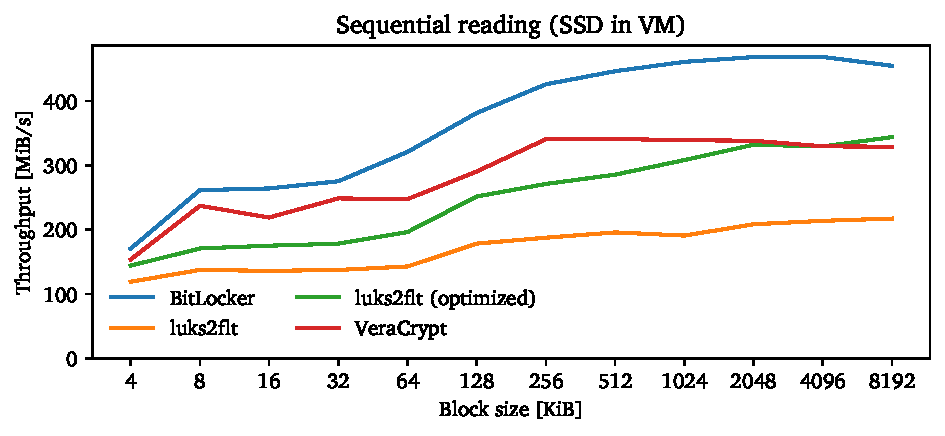
\includegraphics[scale=1]{../fig/performance.vmexperiments.seq.pdf}
	\caption[
		Sequential read rates in the virtual machine
	]{
		Sequential read rates in the virtual machine. The data was obtained by running jobs back to back: one job per combination of driver and block size, grouped by driver and ordered by increasing block size. There was a reboot after the BitLocker, VeraCrypt, and optimized \texttt{luks2flt} jobs to load the less optimized version of \texttt{luks2flt}. Both the \texttt{iodepth} and \texttt{numjobs} parameters were set to a value of 1.
	}
	\label{fig:performance.vmexperiments.seq}
\end{figure}

We observe the following from these results:
\begin{itemize}
	\item BitLocker's sequential read rate is unreachable for both our driver and VeraCrypt at larger block sizes. \todo{concrete values?}
	\item VeraCrypt performs noticeably better at sequential reading than \texttt{luks2flt}'s optimized version, but the difference decreases with increasing block size. VeraCrypt's read rate peaks at 256 KiB, but our driver's rate continues to grow after that.
	\item The more optimized version has a significantly higher sequential read rate than the first version, especially at larger block sizes. At 4 KiB, the increase in performance is about 21\%; at 8192 KiB the more optimized version has about a 59\% higher read rate.
\end{itemize}

\autoref{fig:performance.vmexperiments.rand} shows the random access read rates of the four drivers for different block sizes. BitLocker always has the highest rate, starting at 16 MiB/s and climbing up to 388 MiB/s at 8192 KiB blocks, with a little stagnation and decrease in performance at 256 and 512 KiB. VeraCrypt has the lowest read rate of 10 MiB/s at 4 KiB, but it steadily grows: it rises to third place at 256 KiB, second place at 1024 KiB, and falls back to third at 8192 KiB, with a maximum of 291 MiB/s. The two versions of \texttt{luks2flt} both start at 16 MiB/s and rise for block sizes up to 128 KiB, switching their roles of second and third place. After that, the optimized version continues to improve its read rate up to the final value of 300 MiB/s, temporarily falling behind VeraCrypt. The less optimized version's rate first decreases a bit, then rises abruptly, and then decreasing a bit again, with a maximum value of 144 MiB/s at 1024 KiB.

\begin{figure}[htb!]
	\center
	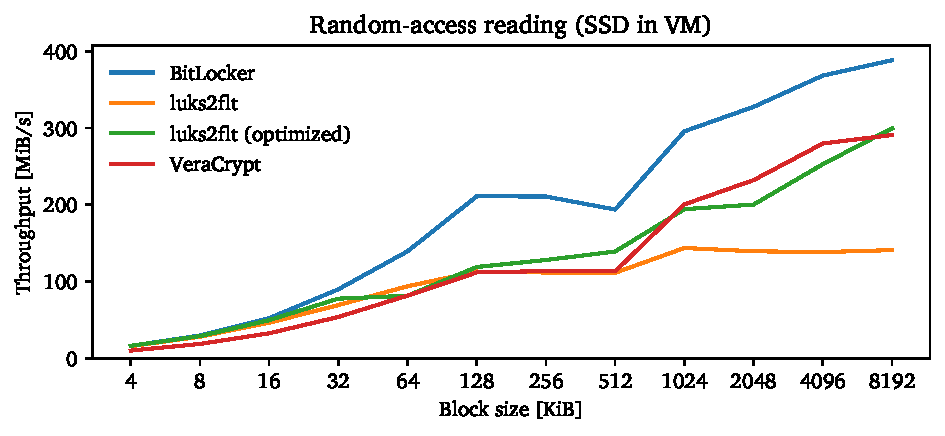
\includegraphics[scale=1]{../fig/performance.vmexperiments.rand.pdf}
	\caption[
		Random-access read rates in the virtual machine
	]{
		Random-access read rates in the virtual machine. See \autoref{fig:performance.vmexperiments.rand} for how we collected the data.
	}
	\label{fig:performance.vmexperiments.rand}
\end{figure}

We observe the following from these results:
\begin{itemize}
	\item BitLocker has the highest random-access read rate, with sometimes almost double the rate of the others (e.g. at 128 KiB).
	\item The optimized version of \texttt{luks2flt} beats VeraCrypt's random-access read rate at two thirds of the tested block sizes. For example, its read rate is 60\% higher at 4 KiB, 52\% higher at 16 KiB, and 14\% lower at 2048 KiB.
	\item Starting from a block size of 128 KiB, the more optimized version has a significantly higher random-access read rate than the first version. For the biggest block size, the more optimized version has a 113\% higher read rate.
\end{itemize}

\paragraph{Interpretation}
Combining our observations from both access patterns, we \todo{draw these conclusions}: \todo{check later if some of these things should maybe be in the discussion instead of here}
\begin{itemize}
	\item BitLocker is the best-performing driver, both at sequential and random-access reading. This is not really surprising, as it is not a fair competition: one driver is the proprietary product of Microsoft, who also wrote the operating system running the driver; and the other two are open source projects by third parties. Microsoft's driver profits from their expertise in Windows' inner workings, and can also take advantage of undocumented internals.
	\item VeraCrypt has a higher sequential read rate than \texttt{luks2flt}, with the difference decreasing for larger block sizes. The former is probably because of VeraCrypt's read ahead caching, as \texttt{luks2flt} does not perform any caching. The latter may be because of VeraCrypt's fragmenting of larger blocks into at most 256 KiB blocks. This means that the I/O performed by the driver can only profit so much from block sizes larger than 256 KiB. This theory is supported by the fact that VeraCrypt reaches its peak sequential read rate at exactly this block size. As already mentioned in \autoref{chap:otherapproaches.veracrypt.peeking}, the fragmenting is done to overlap I/O and cryptographic operations. However, the alleged gains from this overlapping do not seem to be able to cancel out the losses by capping the effective block size at 256 KiB.
	\item For random-access reads, the performance difference between VeraCrypt and \texttt{luks2flt} is smaller, with our driver showing higher read rates most of the time. This supports the thesis that VeraCrypt's performance advantage for sequential access stems from its caching: for random access reads the cache is not effective, and therefore the advantage vanishes.
	\item The changed compiler optimization settings have a significant impact on our driver's read performance, regardless of the access pattern.
\end{itemize}

\paragraph{Another Optimization Attempt}
We also tried optimizing the performance by restricting \texttt{luks2flt}'s cryptographic capabilities to AES-256-XTS and dropping support for AES-128-XTS. This enabled removing some \texttt{if}-\texttt{else} constructs that dispatched de-/encryption functions based on whether AES-128 or AES-256 was used. Even though these conditionals were located in a performance critical section, we found no significant read rate changes. Our theory for why this was the case is the following: in this setup, our driver was only ever used for one LUKS2 partition and therefore always took the same path through the \texttt{if}-\texttt{else} (either always AES-128 or always AES-256). This trained the CPU's branch prediction on this one specific path. Thus, after a short training phase, the CPU always speculatively executed the correct path, resulting in the same performance as without the \texttt{if}-\texttt{else}. The same reasoning applies for a use case where \texttt{luks2flt} is filtering multiple volumes that all use the same AES-XTS variant, \todo{although we did not test this}.

\section{Real Hardware Experiments}
\label{chap:performance.hwexperiments}
After gaining first insights through the virtual machine experiments, we turned to real hardware for a deeper understanding. To combat the issue of variations in read rates due to external circumstances, we did not rely on measurements from single runs. Instead, we ran each job three times and calculated the average read rate. The same job was not run three times back to back; instead, we ran a first series of all jobs, then a second series, and finally a third. Thus, there was always quite some time between running the same job again, which hopefully eliminated most of the external influences.

\subsection{Read Rate Measurements}
\label{chap:performance.hwexperiments.encryptedseries2}
The further optimizations of \texttt{luks2flt}, as described in \autoref{chap:performance.vmexperiments}, unfortunately led to reproducible crashes on real hardware. \todo{(explain that the fastfat driver crashed?)} We consequently disabled some of the optimizations again (Whole program optimization, Spectre mitigations, Link-time code generation, and Frame-pointer omission), and did not find any more crashes. Regrettably, this also led to a performance regression. \todo{check if we can re-enable some options again and increase performance?}

In some of the experiments in this section, multiple threads concurrently executed a job (i.e. \texttt{numjobs} was greater than 1). For these measurements, we took the average of all threads as the read rate for one run of this job. As we ran each job three times, these thread averages were then averaged again to obtain the final read rate for the job.

\todo{no less optimized version of luks2flt any more}

\todo{On HDD, the optimized version of \texttt{luks2flt} generally showed the same trend as on SSD, or even had less read rate differences to the other two drivers.}

\todo{side note: the iodepth=1 and numjobs=1 read rates of BitLocker and VeraCrypt match the ones from the figures with the less optimized luks2flt pretty well. this means that influence of external circumstances is rather low}

\begin{figure}[htb!]
	\center
	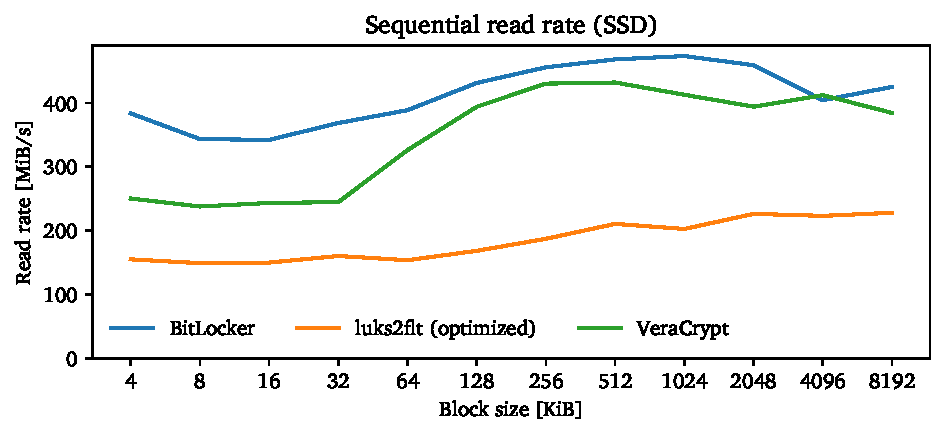
\includegraphics[scale=1]{../fig/performance.hwexperiments.optseq.pdf}
	\caption[
		Sequential read rates
	]{
		Sequential read rates. \todo{todo}
	}
	\label{fig:performance.hwexperiments.optseq}
\end{figure}

\begin{figure}[htb!]
	\center
	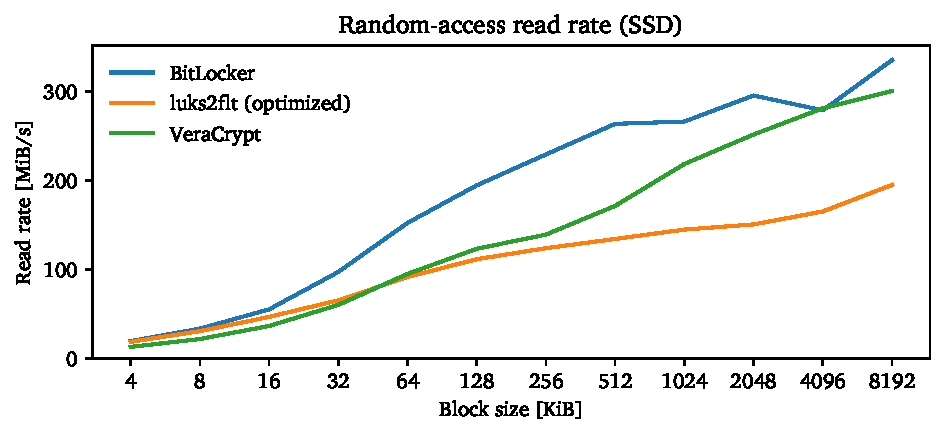
\includegraphics[scale=1]{../fig/performance.hwexperiments.optrand.pdf}
	\caption[
		Random-access read rates
	]{
		Random-access read rates. \todo{todo}
	}
	\label{fig:performance.hwexperiments.optrand}
\end{figure}

\todo{mögliche erklärung für veracrypt's schlechtere performance bei größerer iodepth und numthreads bei random access}: wenn nur ein thread immer nur eine request schickt, dann ist das fragmentieren der request in kleinere blöcke nicht schlimm. aber wenn mehrere requests gleichzeitig abgearbeitet werden, springt der I/O thread hin und her zwischen der abarbeitung von fragmenten aus verschiedenen requests. dh es ist quasi noch mehr random access und auch mit kleinerer block size

\todo{passt diese theorie zu dem was wir bei mehreren requests als sequentielle performance sehen?} ja: der IO thread springt zwar immer noch zwischen fragmenten verschiedener requests hin und her, diese sind aber nicht ansatzweise so weit verteilt wie bei random access. die anfragen liegen bei sequentiellem lesen ja relativ nah beieinander, demnach also auch die fragmente der verschieden anfragen. deswegen leidet veracrypt's performance bei sequentiellem lesen nicht so sehr unter mehreren gleichzeitigen anfragen.

\begin{figure}[htb!]
	\center
	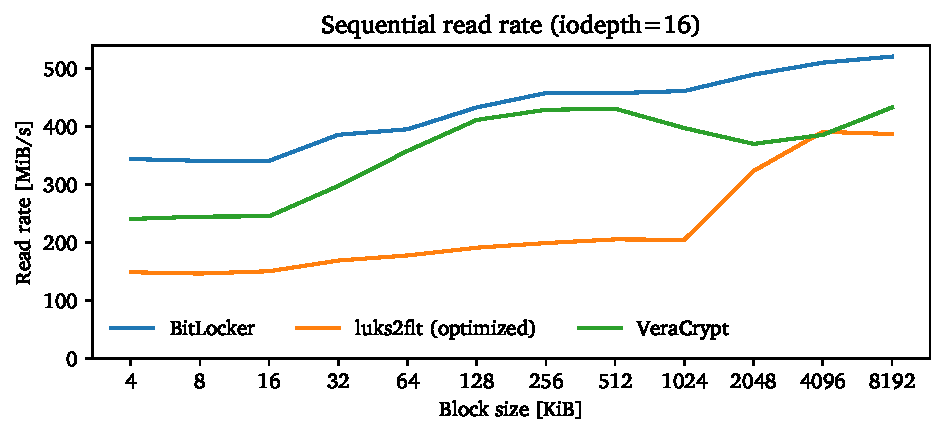
\includegraphics[scale=1]{../fig/performance.hwexperiments.optseqqueue.pdf}
	\caption[
		Sequential read rates with \texttt{iodepth=16}
	]{
		Sequential read rates with \texttt{iodepth=16}. \todo{todo}
	}
	\label{fig:performance.hwexperiments.optseqqueue}
\end{figure}

\begin{figure}[htb!]
	\center
	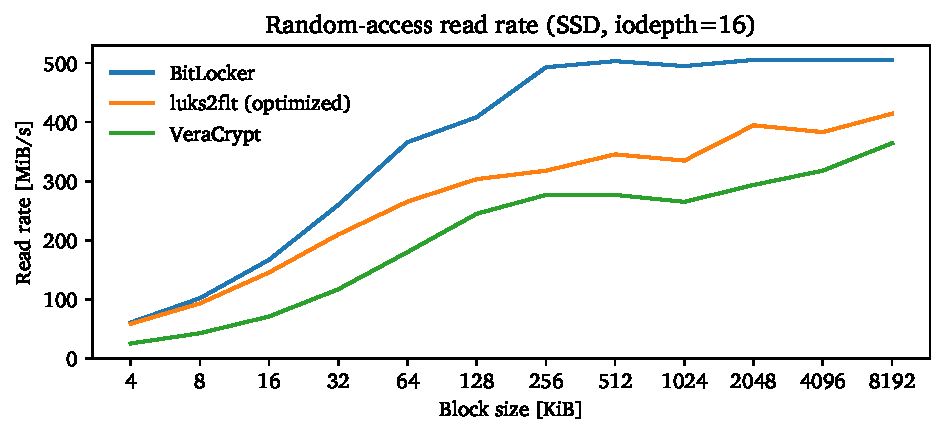
\includegraphics[scale=1]{../fig/performance.hwexperiments.optrandqueue.pdf}
	\caption[
		Random-access read rates with \texttt{iodepth=16}
	]{
		Random-access read rates with \texttt{iodepth=16}. \todo{todo}
	}
	\label{fig:performance.hwexperiments.optrandqueue}
\end{figure}

\begin{figure}[htb!]
	\center
	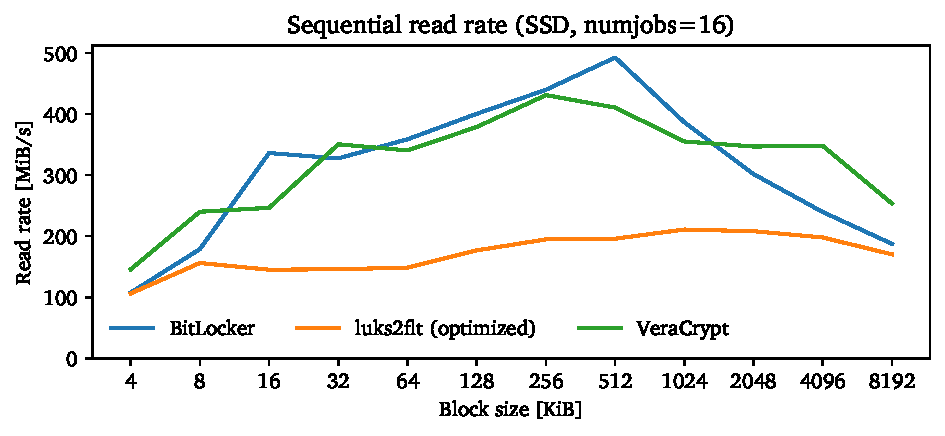
\includegraphics[scale=1]{../fig/performance.hwexperiments.optseqthreads.pdf}
	\caption[
		Sequential read rates with \texttt{numjobs=16}
	]{
		Sequential read rates with \texttt{numjobs=16}. \todo{todo}
	}
	\label{fig:performance.hwexperiments.optseqthreads}
\end{figure}

\begin{figure}[htb!]
	\center
	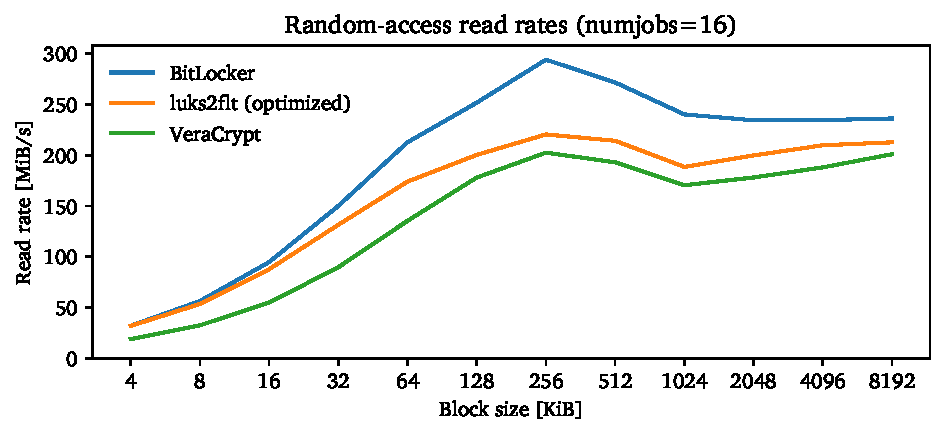
\includegraphics[scale=1]{../fig/performance.hwexperiments.optrandthreads.pdf}
	\caption[
		Random-access read rates with \texttt{numjobs=16}
	]{
		Random-access read rates with \texttt{numjobs=16}. \todo{todo}
	}
	\label{fig:performance.hwexperiments.optrandthreads}
\end{figure}

\begin{figure}[htb!]
	\center
	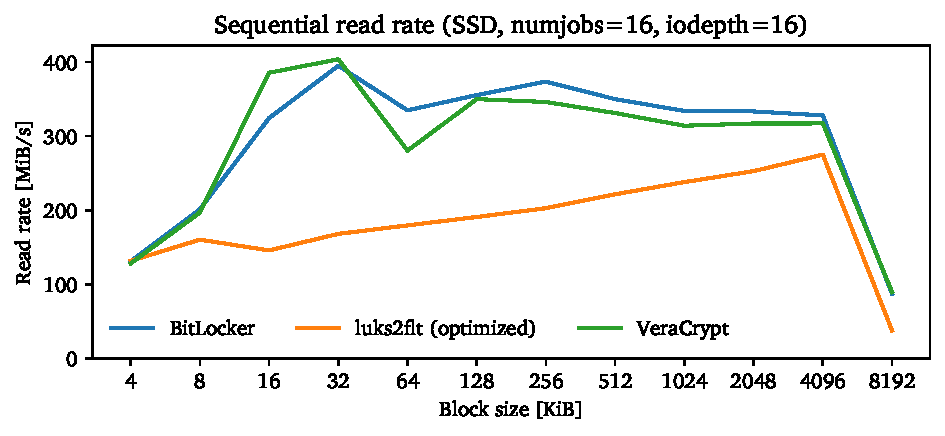
\includegraphics[scale=1]{../fig/performance.hwexperiments.optseqthreadsqueue.pdf}
	\caption[
		Sequential read rates with \texttt{numjobs=16} and \texttt{iodepth=16}
	]{
		Sequential read rates with \texttt{numjobs=16} and \texttt{iodepth=16}. \todo{todo}
	}
	\label{fig:performance.hwexperiments.optseqthreadsqueue}
\end{figure}

\begin{figure}[htb!]
	\center
	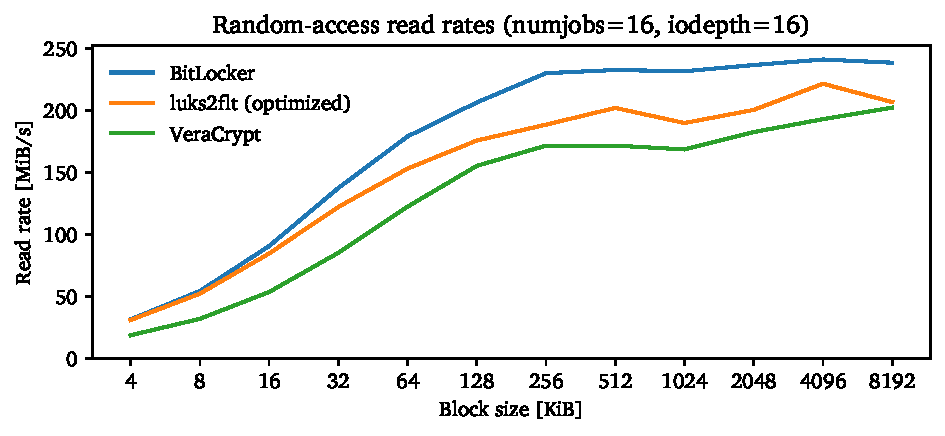
\includegraphics[scale=1]{../fig/performance.hwexperiments.optrandthreadsqueue.pdf}
	\caption[
		Random-access read rates with \texttt{numjobs=16} and \texttt{iodepth=16}
	]{
		Random-access read rates with \texttt{numjobs=16} and \texttt{iodepth=16}. \todo{todo}
	}
	\label{fig:performance.hwexperiments.optrandthreadsqueue}
\end{figure}

\clearpage
\subsection{Measuring Read Rates Over Time}
\label{chap:performance.hwexperiments.readrateovertime}
\texttt{fio} comes with an option to enable the logging of current read rates, \texttt{write\_bw\_log}. By default, one entry in the log file corresponds to one completed I/O request. This is not what we wanted for two reasons: firstly, this does not scale well with larger block sizes, as there are fewer I/O operations when using larger blocks; and secondly, we are not interested in single I/O requests, but the general trend over time (the logs with one line per completed request contain large read rate spikes which we do not care about). Fortunately, there is also an option to log the average bandwidth of the last $N$ milliseconds, where the value of $N$ is configurable: \texttt{log\_avg\_msec}. We found that \todo{16} ms is a good value for this option, yielding data with reasonable high time resolution but not too much spikes from the completion of individual I/O requests.

\begin{figure}[htb!]
	\center
	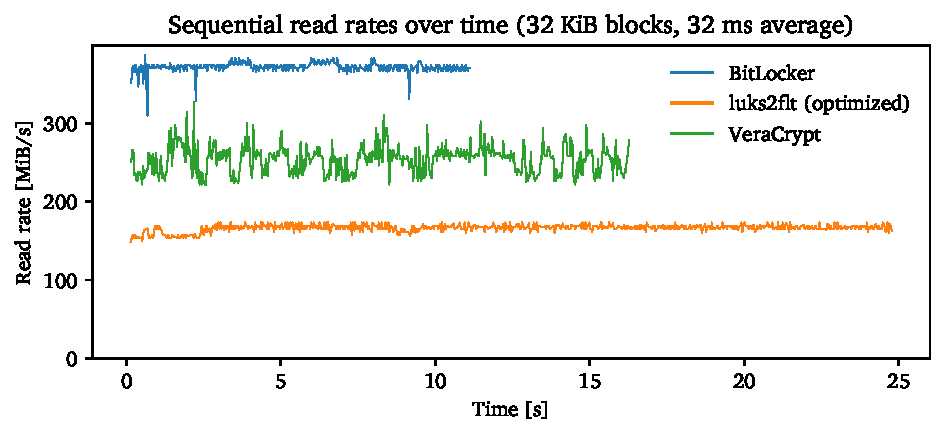
\includegraphics[scale=1]{../fig/performance.hwexperiments.seqovertime.pdf}
	\caption[
		Sequential read rates over time
	]{
		Sequential read rates over time. \todo{todo} \todo{256 KiB blocks, 16 ms average \texttt{iodepth=1}}
	}
	\label{fig:performance.hwexperiments.seqovertime}
\end{figure}

\begin{figure}[htb!]
	\center
	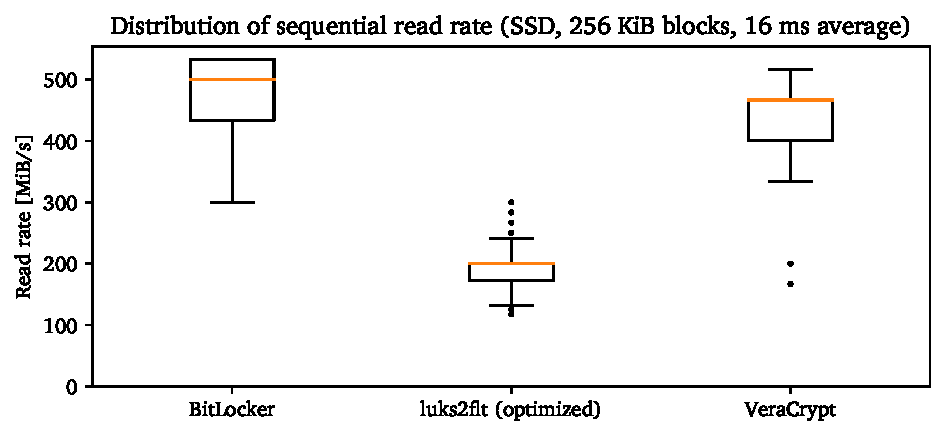
\includegraphics[scale=1]{../fig/performance.hwexperiments.seqovertimebox.pdf}
	\caption[
		Distribution of sequential read rates over time
	]{
		Distribution of sequential read rates over time. \todo{todo} \todo{256 KiB blocks, 16 ms average \texttt{iodepth=1}}
	}
	\label{fig:performance.hwexperiments.seqovertimebox}
\end{figure}

\begin{figure}[htb!]
	\center
	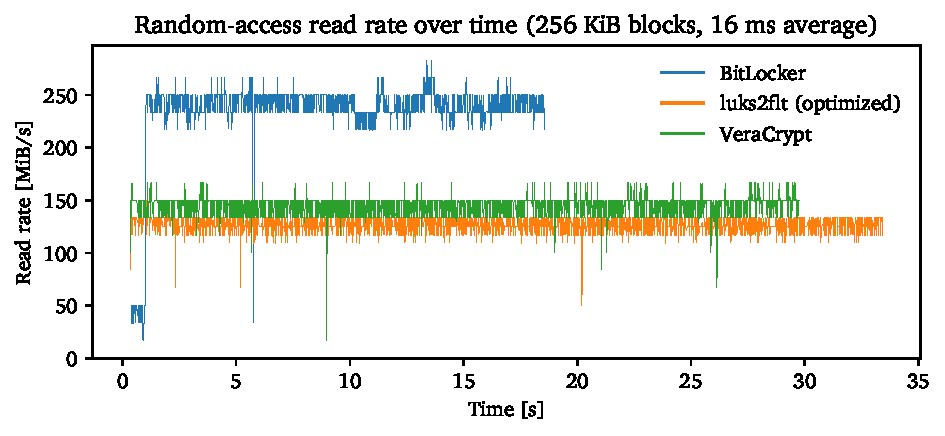
\includegraphics[scale=1]{../fig/performance.hwexperiments.randovertime.pdf}
	\caption[
		Random-access read rates over time
	]{
		Random-access read rates over time. \todo{todo} \todo{256 KiB blocks, 16 ms average \texttt{iodepth=1}}
	}
	\label{fig:performance.hwexperiments.randovertime}
\end{figure}

\begin{figure}[htb!]
	\center
	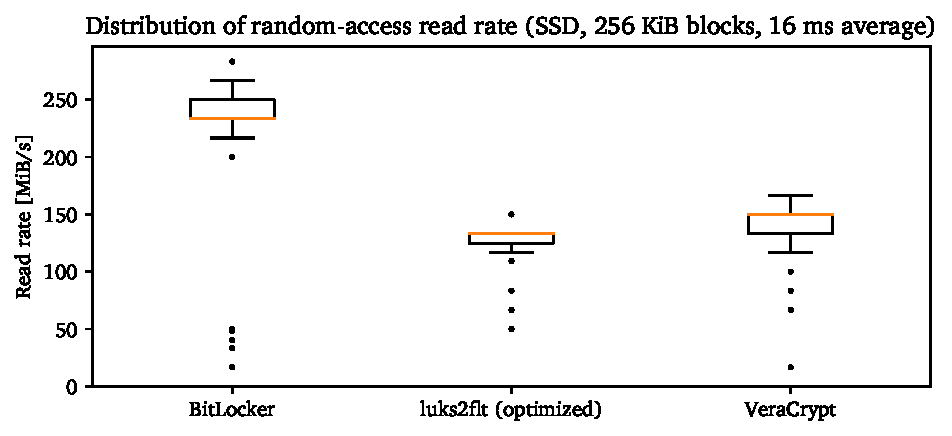
\includegraphics[scale=1]{../fig/performance.hwexperiments.randovertimebox.pdf}
	\caption[
		Distribution of random-access read rates over time
	]{
		Distribution of random-access read rates over time. \todo{256 KiB blocks, 16 ms average \texttt{iodepth=1}}
	}
	\label{fig:performance.hwexperiments.randovertimebox}
\end{figure}

\todo{explain trends for other parameter values (smaller/bigger blocks, ioqueue=16), check how it looks for HDD?}